\label{sec:framework}

\begin{figure*}[t]
    \centering
    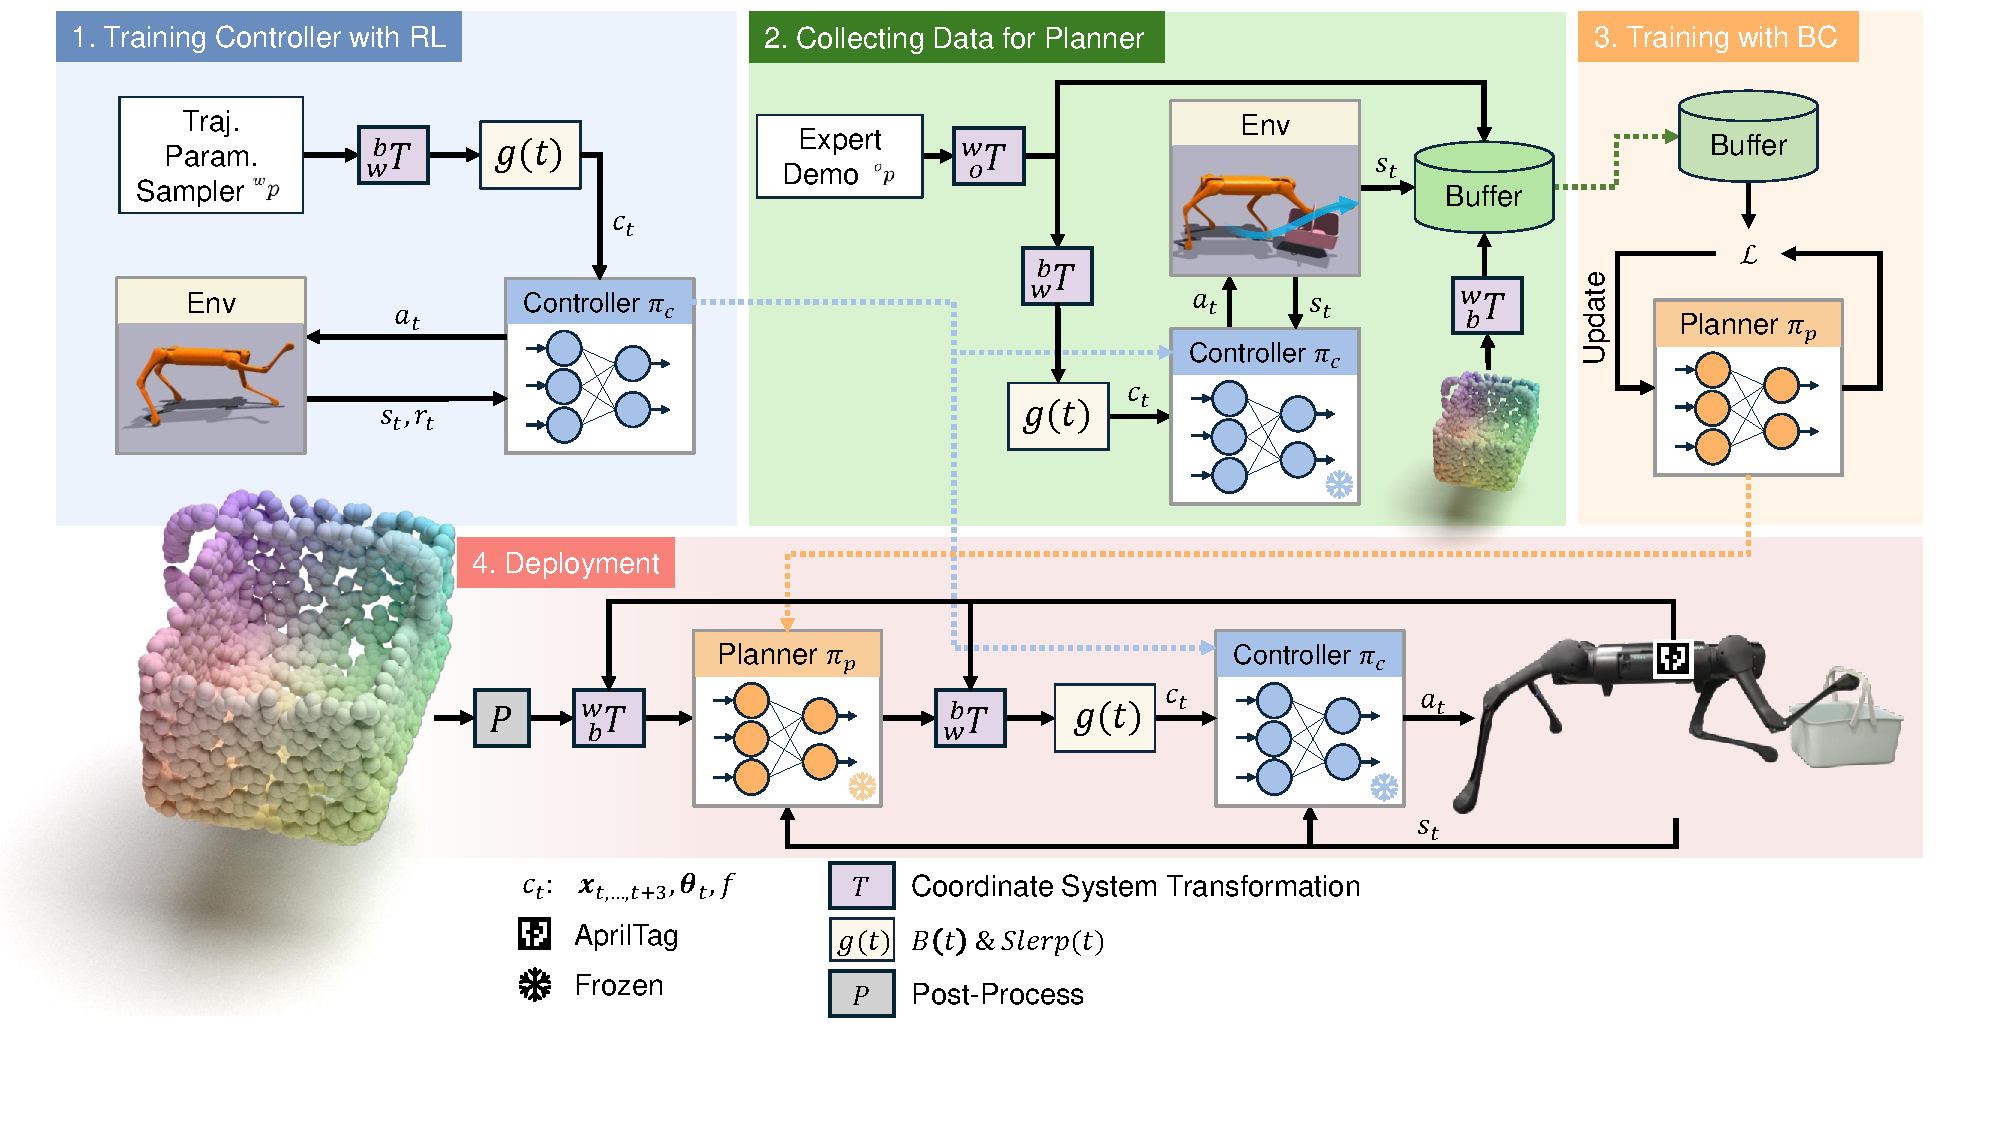
\includegraphics[width=\linewidth, trim={0 15mm 1cm 0}, clip]{figures/framework.pdf}
    \caption{\small (1) We train a control policy $\pi_{c}$ that enables an end-effector to follow curves defined by Bézier control points and weight while maintaining stable locomotion with the other three legs. 
    % We randomize the manipulation trajectory parameters to enable omnidirectional walking and tracking. 
    (2) We use the trained controller to collect expert data. We design manipulation trajectories for different tasks and collect demonstrations through parallel simulation. 
    % 3. During this process, we collect robot states, trajectory parameters in the world frame, and point clouds in the world frame for training the planner. 
    (3) We use the collected expert data and diffusion-based BC to train the planner.
    (4) In the deployment phase, we use the Realsense D435 to obtain the point cloud, and use an external camera to locate the pose of the robot based on AprilTag~\cite{apriltag2011} for trajectory parameter and point cloud coordinate system transformation. These inputs are sequentially fed into the planner and controller, enabling the robot to perform whole-body loco-manipulation tasks.}
    \label{fig:framework}
    \vspace{-0.5cm}
\end{figure*}

In this section, we introduce our hierarchical learning framework, utilizing BC at the high-level manipulation planning and RL at the low-level joint position control, to enable the robot to achieve versatile loco-manipulation skills.

\subsection{Overview}

As illustrated in Fig.~\ref{fig:framework}, motivated by previous work~\cite{ji2023Hierarchical,huang2023creating}, we decompose the loco-manipulation of the robot into two parts: the high-level planner predicts the desired trajectory parameters for the end-effector, while the low-level controller enables the robot to achieve pose tracking with end-effector. 
% The trajectory parameters include the parameters of a rational Bézier curve, the target orientation of the start and end points, and a manipulator flag $f$.
The trajectory parameters define the desired pose of the end-effector and identify the legs functioning as manipulators with a manipulator flag $f$.

To develop the high-level planner $\pi_{p}$, we use the trained control policy $\pi_{c}$ to collect expert demonstration data. Specifically, we design expert trajectory parameters for different tasks and make the robot track them in simulation while collecting robot states, point clouds, and trajectory parameters. Through large-scale parallel simulation, we can collect more than 100 expert demonstrations in 3 minutes. Utilizing the collected expert demonstrations, we develop a high-level planner with DP3~\cite{ze2024DP3}, which takes point clouds and robot states as input and outputs trajectory parameters. The frequency of the high-level planner is $10$ Hz.

We develop a low-level controller $\pi_{c}$, which allows the robot to track a 3-DoF target trajectory with any forelimb while maintaining stable walking. This is achieved by training a policy whose inputs include the manipulator flag, the current desired end-effector pose, the current target point of the end-effector calculated by the rational Bézier curve, and the next three target points. The output is desired robot joint positions $q^{d}_{m} \in \mathbb{R}^{12}$. This control policy runs at $50$ Hz, and the desired torque $\mathbf{\tau}$ of the robot is obtained through a PD controller from the desired joint positions.


% \zli{since lfd is more interesting, put the more interesting thing in the front.}

\subsection{Trajectory Parameterization}
% To maximize the benefits 
To fully capitalize on the strengths of RL and BC and ensure their effective cooperation, we parameterize the manipulation trajectory of the end-effector. 
These trajectory parameters $p$ serve as both the output of the high-level planner and are utilized to calculate the input for the low-level controller.
Our trajectory parameters include the manipulation flag $f$, 6-order rational Bézier curve parameters, and the target orientation of the start and end points, which we further describe below.

\paragraph{Manipulator Flag} We use any one of the forelimbs as the manipulator, which is specified by a binary manipulation flag $f$, where 0 stands for the Front Left (FL) foot and 1 for the Front Right (FR) foot.

\paragraph{Desired Position Trajectory} In this paper, we use rational Bézier curves to represent the manipulation trajectory. 
% This is an extension of the Bézier curve that allows for the
Unlike traditional Bézier curves, which are defined solely by control points, rational Bézier curves introduce adjustable weights for these control points, enabling the
 seamless combination of curves and polylines while still maintaining smoothness by weighting the control points. This enables it to parametrically and flexibly represent different trajectories. We consider the foot toe as the end-effector, and the trajectory of the end-effector in 3D space is specified by rational Bézier curves:
\begin{equation}~\label{eq:bezier}
B_{n}(t)=\frac{\sum_{i=0}^n\binom nit^i(1-t)^{n-i}\mathbf{p}_iw_i}{\sum_{i=0}^n\binom nit^i(1-t)^{n-i}w_i}.
\end{equation}
Where $\mathbf{p}_i \in \mathbb{R}^{3\times1}$ represents the control points, $w_i \in \mathbb{R}$ denotes the weights of the control points, introducing an additional degree of control not present in traditional Bézier curves, and $n+1$ is the number of parameters, with $n=6$ chosen for this paper.


\paragraph{Desired Orientation} 
Our manipulation trajectory uniquely specifies the orientation, a capability not realized in previous work~\cite{cheng2023legmanip, ji2023Hierarchical, arm2024pedipulate}. This advancement enables our robot to execute more complex manipulation tasks.

We employ spherical linear interpolation (SLERP) to calculate the desired orientation, which is a method for smooth interpolation between two orientation vectors:
\begin{equation}~\label{eq:Slerp}
Slerp(\mathbf{q}_{0},\mathbf{q}_{1},t)=\frac{\sin[(1-t)\theta]\cdot \mathbf{q}_{0}+\sin(t\theta)\cdot \mathbf{q}_{1}}{\sin\theta}
\end{equation}
Where $\mathbf{q}_{0}$ represents the target orientation of the starting point, and $\mathbf{q}_{1}$ represents the end orientation of the endpoint. $\theta$ is the angle subtended by the arc. 

In Eq.~\eqref{eq:bezier}and\eqref{eq:Slerp}, $t \in [0,1]$ is the phase time that is scaled according to the time span of the trajectory.

\paragraph{The Choice of Reference Frame for Parameters}

Tracking points directly with a mobile robot in RL can face motion asymmetry issues~\cite{2019-MIG-symmetry, Advanced2022Rudin, hoeller2023anymal}, leading us to use the body frame for trajectory parameters ${}^{b}p$ in our low-level control policy. Our high-level planner operates at a lower frequency than the controller, which could cause tracking errors due to time lags between outputs. To prevent this, we use the world frame for both input point clouds ${}^{w}\mathbf{P}$ and output trajectory parameters ${}^{w}p$, avoiding continuous error corrections and swaying motions. Furthermore, when collecting expert data, we randomize robot and object poses, ensuring trajectory parameters ${}^{o}p$ focus on the object by representing them in the object frame and then converting to the world frame based on the pose of the object.

